\begin{frame}{\tci{} Mid-thesis report}%

    \begin{center}
    %   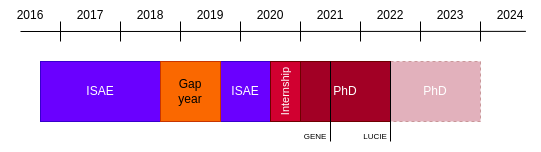
\includegraphics[width=12cm]{images/misc/timeline.drawio.png}

    \tikzset{every picture/.style={line width=0.75pt}} %set default line width to 0.75pt        

        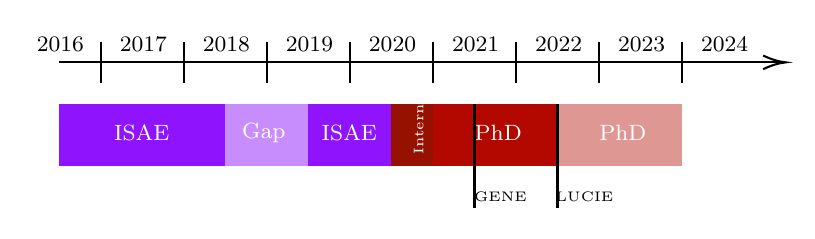
\begin{tikzpicture}[x=0.75pt,y=0.75pt,yscale=-1,xscale=1]
        %uncomment if require: \path (0,300); %set diagram left start at 0, and has height of 300

        %Axis 
        \draw    (80,110) -- (428,110) ;
        \draw [shift={(430,110)}, rotate = 180] [color={rgb, 255:red, 0; green, 0; blue, 0 }  ][line width=0.75]    (10.93,-3.29) .. controls (6.95,-1.4) and (3.31,-0.3) .. (0,0) .. controls (3.31,0.3) and (6.95,1.4) .. (10.93,3.29)   ;
        
        % Years 
        \draw (80.5,101.17) node  [font=\footnotesize] [align=left] {2016};
        \draw    (100,100) -- (100,120) ;
        \draw (120.5,101.17) node  [font=\footnotesize] [align=left] {2017};
        \draw    (140,100) -- (140,120) ;
        \draw (160.5,101.17) node  [font=\footnotesize] [align=left] {2018};
        \draw    (180,100) -- (180,120) ;
        \draw (200.5,101.17) node  [font=\footnotesize] [align=left] {2019};
        \draw    (220,100) -- (220,120) ;
        \draw (240.5,101.17) node  [font=\footnotesize] [align=left] {2020};
        \draw    (260,100) -- (260,120) ;
        \draw (280.5,101.17) node  [font=\footnotesize] [align=left] {2021};
        \draw    (300,100) -- (300,120) ;
        \draw (320.5,101.17) node  [font=\footnotesize] [align=left] {2022};
        \draw    (340,100) -- (340,120) ;
        \draw (360.5,101.17) node  [font=\footnotesize] [align=left] {2023};
        \draw    (380,100) -- (380,120) ;
        \draw (400.5,101.17) node  [font=\footnotesize] [align=left] {2024};
        
        % Blocks
        \draw  [draw opacity=0][fill={rgb, 255:red, 144; green, 19; blue, 254 }  ,fill opacity=1 ] (80,130) -- (160,130) -- (160,160) -- (80,160) -- cycle ;
        \draw  [draw opacity=0][fill={rgb, 255:red, 144; green, 19; blue, 254 }  ,fill opacity=1 ] (200,130) -- (240,130) -- (240,160) -- (200,160) -- cycle ;
        \draw  [draw opacity=0][fill={rgb, 255:red, 200; green, 141; blue, 252 }  ,fill opacity=1 ] (160,130) -- (200,130) -- (200,160) -- (160,160) -- cycle ;
        \draw  [draw opacity=0][fill={rgb, 255:red, 179; green, 8; blue, 0 }  ,fill opacity=1 ] (260,130) -- (320,130) -- (320,160) -- (260,160) -- cycle ;
        \draw  [draw opacity=0][fill={rgb, 255:red, 179; green, 8; blue, 0 }  ,fill opacity=0.42 ] (320,130) -- (380,130) -- (380,160) -- (320,160) -- cycle ;
        \draw  [draw opacity=0][fill={rgb, 255:red, 150; green, 17; blue, 0 }  ,fill opacity=1 ] (240,130) -- (260,130) -- (260,160) -- (240,160) -- cycle ;
        
        % Text
        \draw (120,144) node  [font=\footnotesize,color={rgb, 255:red, 255; green, 255; blue, 255 }  ,opacity=1 ] [align=left] {\begin{minipage}[lt]{20.4pt}\setlength\topsep{0pt}
        ISAE
        \end{minipage}};

        \draw (178.5,144) node  [font=\footnotesize,color={rgb, 255:red, 255; green, 255; blue, 255 }  ,opacity=1 ] [align=left] {\begin{minipage}[lt]{15.64pt}\setlength\topsep{0pt}
        Gap
        \end{minipage}};

        \draw (220,144) node  [font=\footnotesize,color={rgb, 255:red, 255; green, 255; blue, 255 }  ,opacity=1 ] [align=left] {\begin{minipage}[lt]{20.4pt}\setlength\topsep{0pt}
        ISAE
        \end{minipage}};
        
        \draw (253.09,148.63) node  [font=\tiny,color={rgb, 255:red, 255; green, 255; blue, 255 }  ,opacity=1 ,rotate=-270] [align=left] {\begin{minipage}[lt]{8.67pt}\setlength\topsep{0pt}
        Intern
        \end{minipage}};

        \draw (291,144) node  [font=\footnotesize,color={rgb, 255:red, 255; green, 255; blue, 255 }  ,opacity=1 ] [align=left] {\begin{minipage}[lt]{16.32pt}\setlength\topsep{0pt}
        PhD
        \end{minipage}};

        \draw (351,144) node  [font=\footnotesize,color={rgb, 255:red, 255; green, 255; blue, 255 }  ,opacity=1 ] [align=left] {\begin{minipage}[lt]{16.32pt}\setlength\topsep{0pt}
        PhD
        \end{minipage}};

    
        % Papers
        \draw    (280,130) -- (280,180) ;
        \draw (292.5,175) node  [font=\tiny] [align=left] {GENE};
        \draw    (320,130) -- (320,180) ;
        \draw (333,175) node  [font=\tiny] [align=left] {LUCIE};


    \end{tikzpicture}
    \end{center}

    \onslide<2->{
        \begin{block}{Initial topic}
          Bio-inspired methods for artificial neural networks
        \end{block}
      }

    \onslide<3->{
    \begin{block}{Goal of this report}
      Organize past and present work, and highlight future research directions.
    \end{block}
    }
\end{frame}

\begin{frame}{Content}
  \begin{enumerate}%
    \setlength\itemsep{1em}%
    \item<1-> \tci{} \tei{}
    \item<2-> \tcii{} \teii{}
    \item<3-> \tciii{} \teiii{}
    \item<4-> \tciv{} \teiv{}
    \item<5-> \tcv{} \tev{}
    \item<6-> \tcvi{} \tevi{}
  \end{enumerate}
\end{frame}


% \begin{frame}{\tci{} Goals of this defense}
%     \begin{itemize}%
%         \setlength\itemsep{1em}%
%         \item<2-> Present my work so far
%         \item<3-> Look at research directions 
%         \item<4-> Prioritize projects
%     \end{itemize}
% \end{frame}